\begin{frame}{A Note on Standard Error}
    Recall that standard error is closely related to both standard deviation and sample size. In fact,
    \[
        SE = \frac{sd}{\sqrt{n}}
    \]
    This is true regardless of the population parameter of interest.
\end{frame}

\begin{frame}{Confidence Intervals}
    \begin{itemize}
        \item $\hat{p}$ is a single plausible value for the population proportion $p$.
        \item But there is always some standard error associated with $\hat{p}$.
        \item We want to be able to provide a plausible range of values instead.
    \end{itemize}
\end{frame}

\begin{frame}{A Range of Values is Like a Net}
    \begin{itemize}
        \item A point estimate is like spear fishing in murky waters.
        \item Chances are we'll miss our fish.
        \item A range of values is like casting a net.
        \item Now we have a much higher chance of catching our fish.
    \end{itemize}
    This range of values is called a \textbf{confidence interval}.
\end{frame}

\begin{frame}{Confidence Intervals}
    The idea behind a confidence interval is
    \begin{itemize}
        \item Building an interval related to $\hat{p}$
        \item This interval captures a range of plausible values.
        \item With more values come more opportunities to capture the true population parameter.
    \end{itemize}
\end{frame}

\begin{frame}{Confidence Intervals}
    If we want to be very certain that we capture the population parameter, should we use a wider or a smaller interval?
\end{frame}

\begin{frame}{95\% Confidence Intervals}
    \begin{itemize}
        \item Based on our sample, $\hat{p}$ is the most plausible value for $p$.
        \item Therefore will build our confidence interval around $\hat{p}$.
        \item The standard error will act as a guide for how large to make the interval.
    \end{itemize}
\end{frame}

\begin{frame}{95\% Confidence Intervals}    
    \begin{itemize}
        \item When the Central Limit Theorem conditions are satisfied, the point estimate comes from a normal distribution.
        \item For a normal distribution, 95\% of the data is within $|Z|=1.96$ standard deviations of the mean.
        \item Our confidence interval will extend 1.96 standard errors from the sample proportion.
    \end{itemize}
\end{frame}

\begin{frame}{95\% Confidence Intervals}
    Putting these together, we can be 95\% confidence that the following interval captures the population proportion:
    \begin{align*}
        \text{point estimate} &\pm 1.96 \times SE \\
        \hat{p} & \pm 1.96 \times \sqrt{\frac{p(1-p)}{n}}
    \end{align*}
\end{frame}

\begin{frame}{95\% Confidence Intervals}
    In this interval, the upper bound is
    \[
        \hat{p} & + 1.96 \times \sqrt{\frac{p(1-p)}{n}}
    \]
    and the lower bound is 
    \[
        \hat{p} & - 1.96 \times \sqrt{\frac{p(1-p)}{n}}
    \]
\end{frame}

\begin{frame}{95\% Confidence Intervals}
    What does 95\% confident mean?
    \begin{itemize}
        \item Confidence is based on the concept of \textit{repeated sampling}.
        \item Suppose we took 1000 samples and built a 95\% confidence interval from each.
        \item Then about 95\% of these would contain the true parameter $p$.
    \end{itemize}
\end{frame}

\begin{frame}{95\% Confidence Intervals}
    \begin{center}
        \vspace{-20pt}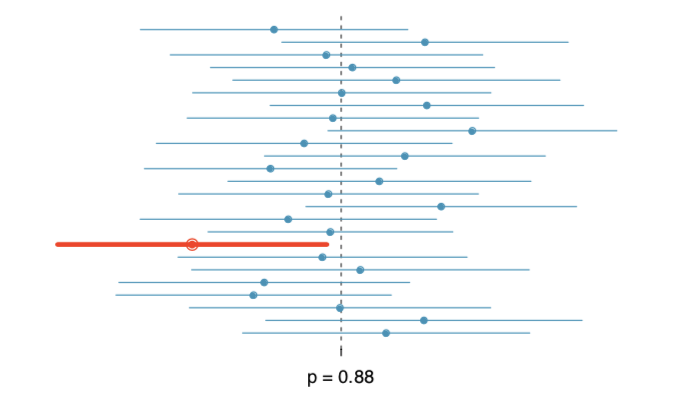
\includegraphics[scale=0.4]{images/manyCIs.png}
    \end{center}
    \vspace{-8pt}\small{25 confidence intervals built from 25 samples where the true proportion is $p=0.88$}. Only one of these did not capture the true proportion.
\end{frame}

\begin{frame}{Example}
    Last class we talked about a sample of 1000 Americans where 88.7\% said that they supported expanding solar power.
    
    \vspace{12pt}Find a 95\% confidence interval for $p$.
\end{frame}

\begin{frame}{Example}
    We decided during our last class that the Central Limit Theorem applies and that
    \[
        \mu_{\hat{p}} = \hat{p} = 0.887
    \]
    and
    \[
        SE_{\hat{p}} = \sqrt{\frac{\hat{p}(1-\hat{p})}{n}} = 0.010
    \]
\end{frame}

\begin{frame}{Example}
    Plugging these into our confidence interval,
    \begin{align*}
        &\hat{p} \pm 1.96 \times SE_{\hat{P}} \\
        &\rightarrow 0.887 \pm 1.96 \times 0.010 \\
        &\rightarrow 0.887 \pm 0.0196 \\
        &\rightarrow (0.8674, 0.9066)
    \end{align*}
    We can be 95\% confident that the actual proportion of adults who support expanding solar power is between 86.7\% and 90.7\%.
\end{frame}

\begin{frame}{More General Confidence Intervals}
    \begin{itemize}
        \item Suppose we want to cast a wider net and find a 99\% confidence interval.  
        \item To do so, we must widen our 95\% confidence interval.
        \item If we wanted a 90\% confidence interval, we would need to narrow our 95\% interval. 
    \end{itemize}
\end{frame}

\begin{frame}{More General Confidence Intervals}
    We decided that the 95\% confidence interval for a point estimate that follows the Central Limit Theorem is
    \[
        \text{point estimate} \pm 1.96 \times SE
    \]
    There are three components to this interval: 
    \begin{enumerate}
        \item the point estimate
        \item “1.96”
        \item the standard error
    \end{enumerate}
\end{frame}

\begin{frame}{More General Confidence Intervals}
    \begin{itemize}
        \item The point estimate and standard error won't change if we change our confidence level.
        \item 1.96 was based on capturing 95\% of the data for our normal distribution.
        \item We will need to adjust this value for other confidence levels.
    \end{itemize}
\end{frame}

\begin{frame}{Consider the Following}
    If $X$ is a normally distributed random variable, what is the probability of the value $x$ being within $2.58$ standard deviations of the mean?
\end{frame}

\begin{frame}{Consider the Following}
    We want to know how often the Z-score will be between -2.58 and 2.58:
    \begin{align*}
        P(-2.58 < Z < 2.58) &= P(Z < 2.58) - P(Z < -2.58) \\
        &= 0.9951-0.0049 \\
        &\approx 0.99
    \end{align*}
    So there is a 99\% probability that $X$ will be within 2.58 standard deviations of $\mu$
\end{frame}

\begin{frame}{99\% Confidence Intervals}
    With this in mind, we can create a 99\% confidence interval:
    \[
        \text{point estimate} \pm 2.58 \times SE
    \]
    All we needed to do was change 1.96 in the 95\% confidence interval formula to 2.58. 
\end{frame}

\begin{frame}{General Confidence Intervals}
    \begin{center}
        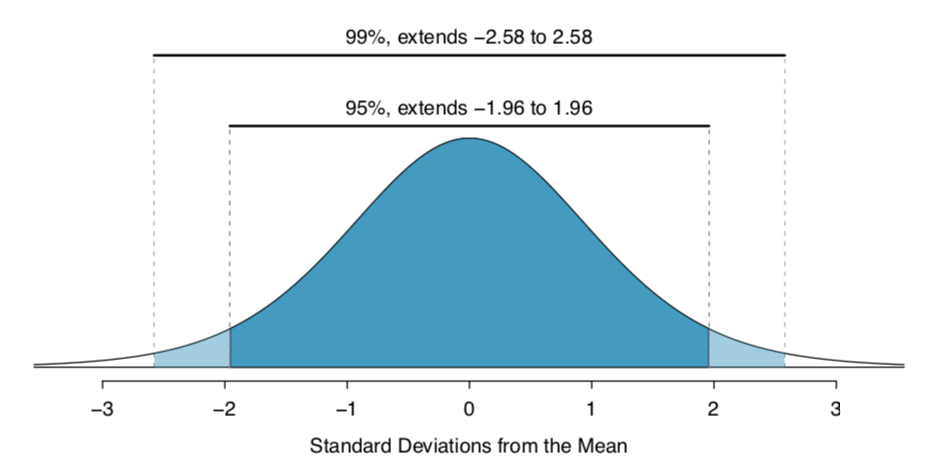
\includegraphics[scale=0.3]{images/zconfs.png}
    \end{center}
    Crucially, the area between $-z_{\alpha/2}$ and $z_{\alpha/2}$ increases as $z_{\alpha/2}$ becomes larger.
\end{frame}

\begin{frame}{What is $\alpha$?}
    For now, we will think of $\alpha$ (Greek letter alpha) as the chance that $p$ is \textit{not} in our interval.
    \[
        \alpha = 1 - \text{confidence level}
    \]
    
    \vspace{12pt}We call $\alpha$ the \textbf{level of significance}.
\end{frame}

\begin{frame}{What is $\alpha$?}
    We can rework our formula for $\alpha$ to say that our confidence level is
    \[
        1-\alpha
    \]
    as a proportion, or 
    \[
        (1-\alpha)\times100\% 
    \]
    as a percent. 
    
    \vspace{12pt}Over the next few slides, we will consider why we use the notation $z_{\alpha/2}$.
\end{frame}

\begin{frame}{General Confidence Intervals}
    \begin{itemize}
        \item Using Z-scores and the normal model is appropriate when our point estimate is associated with a normal model. 
        \item This is true when 
        \begin{enumerate}
            \item our point estimate is the mean of a variable that is itself normally distributed
            \item the Central Limit Theorem holds for our point estimate
        \end{enumerate}
    \end{itemize}
    When a normal model is not a good fit, we will use alternative distributions. These will come up in later chapters.
\end{frame}

\begin{frame}{General Confidence Intervals}
    If a point estimate closely follows a normal model with standard error $SE$, then a confidence interval for the population parameter is
    \[
        \text{point estimate} \pm z_{\alpha/2} \times SE
    \]
    where $z_{\alpha/2}$ corresponds to the desired confidence level.
\end{frame}

\begin{frame}{General Confidence Intervals}
    In this general setting, the upper bound for the interval is
    \[
        \text{point estimate} + z_{\alpha/2} \times SE
    \]
    and the lower bound is
    \[
        \text{point estimate} - z_{\alpha/2} \times SE
    \]
\end{frame}

\begin{frame}{Margin of Error}
    In a confidence interval, 
    \[
        \text{point estimate} \pm z_{\alpha/2} \times SE,
    \]
    we refer to $z_{\alpha/2} \times SE$ as the \textbf{margin of error}.
\end{frame}

\begin{frame}{Margin of Error}
    \begin{itemize}
        \item The margin of error is the maximum amount of error that we allow from the point estimate.
        \item That is, this is the furthest distance from the point estimate that we consider to be plausible.
        \item We expect the true parameter to be within this error, limited by the confidence level.
    \end{itemize}
\end{frame}

\begin{frame}{Margin of Error}
    Margin of error will \textit{decrease} when
    \begin{itemize}
        \item $n$ increases.
        \item $1-\alpha$ decreases.
        \item $\alpha/2$ increases.
        \item $z_{\alpha/2}$ decreases.
    \end{itemize}
    Margin of error will increase under opposite conditions.
\end{frame}

\begin{frame}{Critical Value}
    In a confidence interval, 
    \[
        \text{point estimate} \pm z_{\alpha/2} \times SE,
    \]
    we refer to $z_{\alpha/2}$ as the \textbf{critical value}.
\end{frame}

\begin{frame}{Finding $z_{\alpha/2}$}
    We want to select $z_{\alpha/2}$ so that the area between $-z_{\alpha/2}$ and $z_{\alpha/2}$ in the standard normal distribution, $N(0,1)$, corresponds to the confidence level.
    
    \vspace{12pt}Let $c$ be the desired confidence level. We want to find $z_{\alpha/2}$ such that
    \[
        c = P(-z_{\alpha/2} < Z < z_{\alpha/2})
    \]
\end{frame}

\begin{frame}{Finding $z_{\alpha/2}$}
    Rewriting this,
    \begin{align*}
        c &= P(-z_{\alpha/2} < Z < z_{\alpha/2}) \\
        &= 1 - P(Z > z_{\alpha/2}) - P(Z < -z_{\alpha/2}) \\
    \end{align*}
    Since $Z \sim N(0,1)$ is symmetric,
    \[
        P(Z > z_{\alpha/2}) = P(Z < -z_{\alpha/2})
    \]
\end{frame}

\begin{frame}{Finding $z_{\alpha/2}$}
    So
    \begin{align*}
        c &= P(-z_{\alpha/2} < Z < z_{\alpha/2}) \\
        &= 1 - P(Z > z_{\alpha/2}) - P(Z < -z_{\alpha/2}) \\
        &= 1 - P(Z < -z_{\alpha/2}) - P(Z < -z_{\alpha/2}) \\
        &= 1 - 2P(Z < -z_{\alpha/2}) \\
    \end{align*}
\end{frame}

\begin{frame}{Finding $z_{\alpha/2}$}
    Solving for $P(Z < -z_{\alpha/2})$, we find
    \[
    \frac{1-c}{2} = \frac{\alpha}{2} = P(Z < -z_{\alpha/2})
    \]
    
    Hence $z_{\alpha/2}$!
    
    \vspace{12pt}Since $c$ is some number, say 0.90 (a 90\% confidence level), we now have an easy way to find $z_{\alpha/2}$!
\end{frame}

\begin{frame}{Example: Finding $z_{\alpha/2}$}
    Suppose you want to find a 99\% confidence interval. Find $z_{\alpha/2}$.
    
    \vspace{12pt}We know that
    \[
    \frac{1-c}{2} = P(Z < -z_{\alpha/2})
    \]
    and that a 99\% confidence level translates to $c=0.99$.
\end{frame}

\begin{frame}{Example: Finding $z_{\alpha/2}$}
    So
    \begin{align*}
        P(Z < -z_{\alpha/2}) &= \frac{1-c}{2} \\
        &= \frac{1-0.99}{2}  \\
        &= 0.005
    \end{align*}
    Using software to find this percentile, $-z_{\alpha/2}=-2.58$ (so $z_{\alpha/2} = 2.58$). This is what the textbook told us earlier!
\end{frame}

\begin{frame}{Example}
    Recall our sample of 1000 adults, 88.7\% of whom were found to support the expansion of solar energy. Find a 90\% confidence interval for the proportion. Note that we have already verified conditions for normality.
    
    \vspace{12pt}First, our point estimate is $\hat{p}=0.887$.
\end{frame}

\begin{frame}{Example}
    Now we need to find $z_{\alpha/2}$. Our confidence level is $c=0.90$.
    \begin{align*}
        P(Z < -z_{\alpha/2}) &= \frac{1-c}{2} \\
        &= \frac{1-0.9}{2} \\
        &= 0.05
    \end{align*}
    Using \texttt{R}, we find $-z_{\alpha/2} = -1.65$ (so $z_{\alpha/2}=1.65$). 
\end{frame}

\begin{frame}{Example}
    Then the 90\% confidence interval can be computed as
    \[
        \hat{p} \pm 1.65 \times SE \quad\longrightarrow\quad 0.887 \pm 1.65 \times 0.010
    \]
    which is the interval $(0.8705,0.9035)$. 
    
    \vspace{12pt}Thus we are 90\% confident that 87.1\% to 90.4\% of American adults support the expansion of solar power.
\end{frame}

\begin{frame}{Confidence Interval for a Single Proportion}
    There are four steps to constructing these confidence intervals:
    \begin{enumerate}
        \item Identify $\hat{p}$, $n$, and the desired confidence level.
        \item Verify that $\hat{p}$ is approximately normal 
        \begin{itemize}
            \item Use the success-failure condition with $\hat{p}$ to verify the Central Limit Theorem.
        \end{itemize}
        \item Compute $SE$ using $\hat{p}$ and find $z_{\alpha/2}$, using these values to construct your interval.
        \item Interpret your confidence interval \textit{in the context of the problem}.
    \end{enumerate}
\end{frame}

\begin{frame}{Example: Ebola}
    After a doctor contracted Ebola in New York City, a poll of 1042 New Yorkers found that 82\% were in favor of a mandatory quarantine for anyone who'd come in contact with with an Ebola patient.
    
    \vspace{12pt}We will walk through developing and interpreting a 95\% confidence interval for the proportion of New Yorkers who favor mandatory quarantine.
\end{frame}

\begin{frame}{Example: Ebola}
    First, we need to find the point estimate and confirm that a normal model is appropriate.
    \[
        \hat{p} = 0.82
    \]
    This is the given proportion of polled New Yorkers who favored mandatory quarantine.
\end{frame}

\begin{frame}{Example: Ebola}
    To confirm that a normal model is appropriate, we check our success-failure condition using the plug-in approach:
    \[
        n\hat{p} = 1042\times0.82 = 853.62 \ge 10
    \]
    and 
    \[
        n(1-\hat{p}) = 1042\times(1-0.82)= 187.38 \ge 10
    \]
\end{frame}

\begin{frame}{Example: Ebola}
    Since the normal model is appropriate, we can move on to calculating the standard error for $\hat{p}$ based on the Central Limit Theorem. We will again use the plug-in approach.
    \[
        SE_{\hat{p}} \approx \sqrt{\frac{\hat{p}(1-\hat{p})}{n}} = \sqrt{\frac{0.82(1-0.82)}{1041}} = 0.012
    \]
\end{frame}

\begin{frame}{Example: Ebola}
    Now we want to find our critical value $z_{\alpha/2}$ for our 95\% confidence interval. In this case,
    \[
        \alpha = 1-\text{confidence level} = 0.05
    \]
\end{frame}

\begin{frame}{Example: Ebola}
    Then, using software, $z_{\alpha/2}=z_{0.025}=1.96$ and our confidence interval is
    \begin{align*}
        \hat{p}\pm z_{\alpha/2}\times SE &= 0.82 \pm 1.96 \times 0.012 \\
        &= 0.82 \pm 0.0235
    \end{align*}
    or $(0.796, 0.844)$.
\end{frame}

\begin{frame}{Example: Ebola}
    Finally, to interpret the interval $(0.796, 0.844)$:
    
    \vspace{12pt}We can be 95\% confident that the proportion of New York adults in October 2014 who supported a quarantine for anyone who had come into contact with an Ebola patients was between 0.796 and 0.844.
\end{frame}

\begin{frame}{Example: Ebola}
    When we say that we are 95\% confident, we mean:
    
    \vspace{12pt}If we took many such samples and computed a 95\% confidence interval for each
    \begin{itemize}
        \item About 95\% of those intervals would contain the actual proportion.
        \item This proportion is of New York adults who supported a quarantine for anyone who has come into contact with an Ebola patient.
    \end{itemize}
\end{frame}

\begin{frame}{Interpreting Confidence Intervals}
    Whenever we interpret a confidence interval,
    \begin{enumerate}
        \item The statement should be about the population parameter of interest.
        \item We do \textit{not} want to talk about the probability that that interval captures the population parameter.
        \begin{itemize}
            \item This is an important technical detail that has to do with our definition of "95\% confident".
        \end{itemize}
    \end{enumerate}
\end{frame}

\begin{frame}{Interpreting Confidence Intervals}
    Whenever we interpret a confidence interval,
    \begin{enumerate}\setcounter{enumi}{2}
        \item The confidence interval says nothing about individual observations or point estimates.
        \item These methods apply to sampling error and ignore bias entirely!
        \begin{itemize}
            \item If we are systematically over- or under-estimating, confidence intervals will not address this problem.
        \end{itemize}
    \end{enumerate}
\end{frame}

\begin{frame}{Example: Interpreting Confidence Intervals}
    Consider the 90\% confidence interval for the solar energy survey: 87.1\% to 90.4\%. If we ran the survey again, can we say that we’re 90\% confident that the new survey’s proportion will be between 87.1\% and 90.4\%?
\end{frame}

\begin{frame}{Example: Interpreting Confidence Intervals}
    No! Confidence intervals don't tell us anything about future point estimates.
    
    \vspace{12pt}Our point estimate will change so our confidence interval will change.
\end{frame}